\RequirePackage{snapshot}
% Snapshot is required for bundledoc
% Use bundledoc on the merged .tex file (see Makefile; flatex)
% pdflatex merged.tex
% bibtex merged.tex
% pdflatex merged.tex
% bundledoc --config=file.cfg merged.dep
% You have added two cfg files. One uses zip, but there must be a bug
% in bundledoc because the zip file is not deleted from /tmp and not
% moved to the workind directory. The file seems fine so I think
% you can just move it manually. The other cfg file works but
% produces a tar.gz file which is not convenient for Biochemistry
% submission.
\documentclass[12pt]{article}

\usepackage{amsmath,amsfonts,amssymb,amsthm,booktabs,array,mathtools}
\usepackage[version=3]{mhchem}
\usepackage{graphicx}
\usepackage{rotating} % make your own prime symbol
\usepackage{adjustbox} % make your own prime symbol
\usepackage[scaled=1.2]{inconsolata} % monospaced font for sequences

\usepackage{color} % for the pdf + latex export
\usepackage{transparent} % for the pdf + latex export
\usepackage{import}

%\listfiles

\newcommand*{\ppp}{\adjustbox{raise=0.4ex, right=0.56ex}{\scalebox{0.7}{$'$}}\;}

\author{J\o rgen Skancke}

\title{Kinetics of abortive transcription initiation}

\begin{document}

%%%%%%%%%%%%%%%%%%%%%%%%%%%%%%%%%%%%%%%%%%%%%%%%%%%%%%%%%%%%%%%%%%%%%
%% The abstract environment will automatically gobble the contents
%% if an abstract is not used by the target journal.
%%%%%%%%%%%%%%%%%%%%%%%%%%%%%%%%%%%%%%%%%%%%%%%%%%%%%%%%%%%%%%%%%%%%%
% max 250 words for biochemistry
\begin{abstract}
In the initial stage of gene expression, promoter-bound RNA polymerase (RNAP)
goes through repeated cycles of abortive RNA synthesis before reaching
promoter escape. In contrast to transcription elongation, where RNAP moves
along the DNA template, initial transcription requires DNA to be pulled into
the enzyme via the mechanism of scrunching. This is thought to result in
strain in the initial transcribing complex, which may contribute to abortive
RNA release and promoter escape. Here, we investigate the kinetics of initial
transcription on the N25 promoter using a novel method that uses abortive
probabilities from bulk experiments to calculate the rate constants of
backtracking. Applying this method within a parameter estimation scheme, where
we fit the model to the time RNAP spends in abortive cycles as obtained from
single molecule experiments, we identify the rate constants for the nucleotide
addition cycle and the steps of unscrunching and abortive RNA release. Our
results suggest that promoter-bound transcription proceeds at the same speed
as for transcription elongation. This implies that the strain caused by
scrunching does not affect the speed of initial transcription. The best fit by
the model to experimental data shows that the time RNAP spends in abortive
cycling does not follow an exponential distribution for abortive cycles
shorter than 3.5 seconds, as had been previously suggested. Rather, a
time-delay for transcribing the first 11 basepairs must be considered. We
conclude that the rate limiting step for initial transcription is unscrunching
and abortive RNA release, in agreement with experimental evidence. 

\end{abstract}

%%%%%%%%%%%%%%%%%%%%%%%%%%%%%%%%%%%%%%%%%%%%%%%%%%%%%%%%%%%%%%%%%%%%%
%% Start the main part of the manuscript here.
%%%%%%%%%%%%%%%%%%%%%%%%%%%%%%%%%%%%%%%%%%%%%%%%%%%%%%%%%%%%%%%%%%%%%
\section{Introduction}
%\addbibresource{/home/jorgsk/Dropbox/phdproject/bibtex/jorgsk.bib}
Transcription of DNA is at the core of cellular metabolism and a highly
regulated process at multiple levels. In bacteria, transcription is performed
by a single RNAP, which when associated with a $\sigma$ factor can identify
and bind to promoter regions of DNA, forming a DNA bubble and the RNAP-DNA
open complex. RNAP is still bound to the promoter during the first steps of
RNA synthesis and its translocation occurs by the mechanism of scrunching
\cite{revyakin_abortive_2006, kapanidis_initial_2006}, where DNA is pulled
into RNAP to expose the enzyme's active site for NTP binding. This causes the
DNA bubble to grow by one base pair for each NTP added to the RNA's growing
3\ppp end, until it has synthesized an RNA of 8-15 nt in length,
\cite{carpousis_cycling_1980,hsu_vitro_2003,tang_real-time_2009,hsu_initial_2006},
where it may break promoter bonds,  entering the phase of productive
transcription elongation. However, not all initial transcription attempts
result in promoter escape. At any position before escape is reached, RNAP may
instead release the nascent RNA and fall back to the open complex formation,
from where transcription may be re-initiated \cite{carpousis_cycling_1980}.
The process of repeated RNA synthesis and abortive release is known as
abortive cycling. It has been shown that the extent of abortive cycling
depends on the sequence context of both the core promoter region and the
initial transcribed sequence (ITS) \cite{hsu_initial_2006, hsu_promoter_2002,
vo_vitro_2003}.

The complete picture of the mechanisms involved in initial transcription is
not fully understood. In particular, the reaction steps that precede abortive
RNA release, and their kinetics, have not yet been determined. For instance, we
do not know whether the speed of transcription differs between the promotor
bound stage (translocation by scrunching) and the elongating stage
(translocation by base-stepping). To fully understand transcription
regulation, we need to further explore the dynamics of initial transcription. 

It is known so far that some or all abortive RNA releases are associated with
the step of backtracking. This step constitutes a reverse motion where RNAP
releases scrunched DNA, forcing the nascent RNA 3\ppp end to extrude into the
NTP entry channel. Backtracking is strongly associated with abortive RNA
release, since the amount of abortive product is reduced in the presence of
GreB, a protein that rescues backtracked complexes by stimulating RNAP's
intrinsic RNA cleavage activity
\cite{hsu_initial_2006,hsu_escherichia_1995,feng_grea-induced_1994}.

The current conceptual model of abortive cycling consists of the progressive
steps of scrunching and nucleotide addition (together referred to as the
nucleotide addition cycle, NAC), and the regressive steps of backtracking,
unscrunching, and abortive RNA release. Early kinetic work with bulk
transcription experiments on the \textit{lac} UV5 promoter showed a half-life
of full length RNA synthesis on short DNA templates of 1 minute, and that
promoter-binding was not the rate-limiting step \cite{stefano_lac_1979}. Given
the short length of the templates, this implied a rate-limiting step between
promoter binding and promoter escape. It was soon after shown that the
time-delay for full length RNA synthesis coincided with the synthesis of large
quantities of short abortive transcripts, which implied abortive cycling as
the rate limiting step \cite{munson_abortive_1981}. Recent knowledge about the
kinetics of initial transcription has come largely from single-molecule
experiments \cite{revyakin_abortive_2006, kapanidis_initial_2006,
tang_real-time_2009, kapanidis_retention_2005, margeat_direct_2006}. For
bacterial RNAP, it has been found that the backtracking and abortive RNA
release steps are slow relative to forward translocation and RNA synthesis
\cite{revyakin_abortive_2006, margeat_direct_2006}, but so far the exact
kinetic difference of these steps has not been quantified. The most detailed
description of the kinetics of initial transcription in bacteria is the
characterization of the time RNAP spends in abortive cycling on the N25
promoter in the presence of GreB \cite{revyakin_abortive_2006}. This work
showed that RNAP spends between 3 and 20 seconds in abortive cycling over a
stretch of 11 bp of DNA before achieving promoter escape
\cite{revyakin_abortive_2006}.

By proposing the rate limiting steps and finding the distribution of time
spent in abortive cycling, single-molecule experiments have revealed a general
kinetic picture of initial transcription. However, their time-resolution has
not yet been sufficient for distinguishing the rate constants for the
individual steps of backtracking, unscrunching, and abortive RNA release. Moreover,
while these methods have been used to quantify the speed of transcription for
transcription elongation \cite{wang_force_1998,
tolic-norrelykke_diversity_2004}, their relatively low temporal resolution
have yet not allowed the identification of the speed of the NAC during initial
transcription \cite{revyakin_abortive_2006, margeat_direct_2006}.

Although single-molecule experiments can reveal highly detailed information
about the movement and position of single RNAPs during initial transcription,
traditional bulk experiments must still be used to quantify the relative molar
abundance of abortive transcripts. By knowing the relative abundance of each
abortive RNA species, one may calculate the probability of producing an
abortive transcript of any given length, known as the abortive probability
(AP) \cite{hsu_promoter_2002, hsu_quantitative_1996}. Since backtracking is a
starting point for abortive RNA releases, bulk transcription experiments
therefore provide a position-specific indication of the likelihood of
backtracking during initial transcription. In the present study, we have
created a kinetic model of initial transcription that combines the abortive
probabilities obtained from steady state bulk experiments with
time-distribution of abortive cycling from single-molecule experiments. We
inferred from this model the rate constants for the NAC and the combined step
of unscrunching and abortive RNA release. Our results indicate two important
notions: 1) the speed of the NAC is the same for promoter-bound RNAP as
for promoter-free RNAP following promoter escape, and 2) the rate of NAC is 10
times faster than the unscrunching and abortive RNA release, confirming the
results from other studies that have suggested that these steps are
rate limiting for promoter escape.


\section{Materials and Methods}
%\addbibresource{/home/jorgsk/Dropbox/phdproject/bibtex/jorgsk.bib}
\SUBSECTION{Model of initial transcription}
Our model describes the process of initial transcription by considering the
following reactions: i) the NAC ii) backtracking iii) unscrunching and abortive
RNA release (UAR), and iv) promoter escape (\FIG~\ref{fig:model_and_rates}).
We consider backtracking as the first unscrunching step, also known as
backstepping. To find the rate constant of
backtracking we emply a novel method which makes use of abortive probabilities
(APs) calculated from experimental data \cite{hsu_quantitative_1996}. The
method relies on two key points. The first is the model constraint that the
reactions of the NAC and backtracking are in kinetic competition. The second
is the assumption that the probability to backtrack at any given template
position is equal to the AP at that position. Thus we get
\begin{equation*}
    \frac{b_i}{b_i + \text{NAC}_i} = \text{AP}_i,
\end{equation*}
where subscript $i$ indicates position, and NAC and $b$ are the rate constants
the nucleotide addition cycle and backtracking, respectively. From this
expression, we obtain the rate constant for backtracking given a rate constant
of the NAC and an AP:
\begin{equation}
  b_i = \frac{\text{NAC}_i\cdot\text{AP}_i}{1-\text{AP}_i}.
  \label{eq:backtrackingcalc}
\end{equation}
\FIG~\ref{fig:model_and_rates} shows an example calculation of rate constants
of backtracking using NAC = 10 $s^{-1}$.

In this work we run model simulations alternately using APs obtained both for
the absence of GreB (-GreB) and in the presence of GreB (+GreB). When GreB is
present, we note that backtracked complexes may be rescued by GreB stimulated
cleavage of the unaligned 3\ppp end of the transcript. Therefore, APs obtained
in the presence of GreB represent the probability to both backtrack and to
avoid rescue by GreB until abortive RNA release. We therefore assume that
GreB-mediated cleavage and subsequent NACs are rapid steps compared to
unscrunching. This permits using the APs obtained in the presence of GreB as
effective backtracking probabilities. All AP values used in this work are
obtained from Hsu et al. \cite{hsu_initial_2006}.

\SUBSECTION{Implementation and rate constant estimation}
A central result in this work is determining the model rate constants. We do
this running multiple simulations with different combinations of rate
constants and fitting to exeprimental data. The data used for rate constant
estimation is the distribution of time spent in abortive cycling on the N25
promoter in the presence of $100\ \mu M$ NTP determined by Revyakin et al.\
\cite{revyakin_abortive_2006}. This data was obtained from 100 individual
initial transcription events. For experiments with single molecules, there is
an inherent stochastic component in the experimental outcome that derives from
the randomness of molecular motion. That this is evident for transcription can
be inferred from the large variation observed in single-molecule experiments
of the speed of transcription elongation \cite{adelman_single_2002,
tolic-norrelykke_diversity_2004}. To account for this randomness, we perform
the kinetic simulations using the Gillespie algorithm for stochastic
simulations of chemical reactions \cite{gillespie_exact_1977}. Specifically,
we make use the version implemented by Maarleveld et al.\ in the StocPY
software \cite{maarleveld_stochpy:_2013}.

The proceedure for rate constant estimation (illustrated in
\FIG~\ref{fig:model_and_rates}) is as follows (rate constant names indicated
in \FIG~\ref{fig:model_and_rates}): First, we assign random values to the
three rate constants NAC ($k_n$), promoter escape ($k_e$) and unscrunching and
abortive RNA release ($k_u$) within certain fixed boundaries (see below).
These values are chosen independently from a uniform distribution. Secondly,
we use the rate constant of the NAC and the APs to calculate the rate constant
of backtracking ($k_b$) using Eq.~(\ref{eq:backtrackingcalc}). We then
simulate 100 initial transcription events and calculate the distribution of
time spent in abortive cycling as a result of these specific rate constants.
The result is measured against the empirical distribution
\cite{revyakin_abortive_2006} using the root mean square error. By repeating
this procedure several times, we obtain statistics of which values of rate
constants that are associated with the best match with the experimental data.
By virtue of using stochstic simulations, one does not arrive at a unique set
of rate constants that have optimal fit with data; if a simulation is repeated
without changing the rate constants, slightly different results will be
obtained due to the inherent stochastisity of the reaction process. Therefore,
we here find the optimal rate constants by running multiple simulations and
identifying the rate constants that are most often associated with best fit to
data from the distribution of fitness.

The boundaries of the rate constants for parameter estimation were chosen from
extrema estimated from experimental data. The speed of the NAC during initial
transcription cannot be much less than 3 nt/s, since Revyakin et al.\ measured
3.5 seconds as the shortest duration of abortive cycling
\cite{revyakin_abortive_2006} to cover the ~ 11 nt/s required for promoter
escape on N25. At the same time, it should not be larger than at most 25 nt/s,
which is at the upper limit of measured values from single-molecule
experiments \cite{bai_mechanochemical_2007}. While it is not clear how
transcription would proceed faster for promoter-bound RNAP, we use 25 nt/s as
a maximum value also in order to see if the model is able to discard these
values during rate constant estimation. For backtracking and abortive RNA
release, it is known that the rate constant must be faster than 1 s$^{-1}$,
this was the time-resolution of the experimental equipment and this reaction
step could not be resolved \cite{revyakin_abortive_2006}. We therefore set the
minimum and maximum values of all rate constants to be 1 s$^{-1}$ and 25
s$^{-1}$, respectively. 

\begin{figure}[h]
  \caption{{\bf Kinetic scheme of initial transcription on the N25 promoter.}
    From the open complex (OC) transcription proceeds by NACs from one initial
    transcribing complex (ITC) to the next, where each ITC is identified in
    subscript by the length of its nascent RNA. Initial transcription proceeds
    until the nascent RNA has reached the experimentally obtained maximum size
    of abortive transcript; here 11 nt \cite{hsu_initial_2006}. For ITCs with
    an RNA of 2 nt in length or longer, there is a competition between the the
    NAC and backtracking. Backtracking causes termination of transcription,
    and only further backtracking (unscrunching) and abortive RNA release may
    follow, returning RNAP to the open complex. From the open complex forward
    transcription may resume once more. The names of the rate constants are as
    follows: $k_n$ (NAC), $k_e$ (promoter escape), $k_u$ (unscrunching and
    abortive RNA release) and $k_{b,i}$ (backtracking).}
    \label{fig:model_and_rates}
\end{figure}


\section{Results}
%\addbibresource{/home/jorgsk/Dropbox/phdproject/bibtex/jorgsk.bib}
\SUBSECTION{Transcription proceeds at a similar average speed for initial
transcription as for transcription elongation}

We identified the rate constants for initial transcription using a two-step
method (see Methods). We found in the first step that the rate constant for
NAC is greater than 6/s; that the rate constant for unscrunching and abortive
RNA release lies between 1/s and 3/s; and that the rate constant for promoter
escape is greater than 2.3/s
(\FIG~\ref{fig:parameter_estimation_two_iterations}A). The distribution for the
promoter escape rate constant (right panel) did not exhibit any optimal peak,
which indicates that the time that RNAP spends in abortive cycling is not
sensitive to the rate constant for promoter escape. This is reasonable since
the reaction for promoter escape occurs downstream the sequence and does not
affect the duration of abortive cycling.   

In the second step, we varied the rate constant for the NAC between 6/s and
14/s, and UAR between 1/s and 3/s, based on the distributions of these values
from the first step (\FIG~\ref{fig:parameter_estimation_two_iterations}A). Because it
did not affect abortive cycling, we fixed the rate constant of promoter escape
to 20/s. The top 1\% best fitting results from the second round of estimation
resulted in clear peaks in the distributions for both rate constants. The rate
constant for the NAC showed a peak at 10.6/s
(\FIG~\ref{fig:parameter_estimation_two_iterations}B), consistent with the measured
speed of elongating RNAP (9.2 nt/s on positively supercoiled DNA and 13.3 nt/s
on negatively supercoiled DNA \cite{revyakin_abortive_2006}). The rate constant
for UAR peaked at 1.4/s, nearly 10 times slower than the NAC. This low value is
consistent with experimental evidence, suggesting that unscrunching and
abortive RNA release are rate limiting for initial
transcription~\cite{revyakin_abortive_2006, margeat_direct_2006}. Overall, the
rate constants we estimated resulted in an accurate predictive model where most
experimental measurements fell within one standard deviation of the mean model
prediction (\FIG~\ref{fig:revyakin_fit}). 

\SUBSECTION{Short duration scrunching does not follow an exponential distribution}
  
Our model predicts that less than 4\% of scrunching events are shorter than
one second (\FIG~\ref{fig:revyakin_fit}). These quick events represent RNAP
transcribing the 11 required base pairs for promoter escape without
backtracking with a NAC $k_n$ of 10.6/s
(\FIG~\ref{fig:revyakin_fit}). This prediction is lower than the 20\%
predicted previously from extrapolation of data
(\cite{revyakin_abortive_2006}).  

To test the validity of our predictions, we first assumed that the previous
prediction, obtained by extrapolation of an exponential fitting
curve to measurements, was accurate. We then repeated the parameter
estimation (see Methods) but now the RMSE was calculated by the predicted
$\hat T$ from the fitted curve, not the data measurements (see also
\FIG~\ref{fig:param_estimation_scheme} and Algorithm 1). Fitting to the
extrapolated data resulted in an overestimated rate constant for the NAC
($k_n= 23.4$/s). Not only that this $k_n$ value is twice as high as that
reported for transcription elongation \cite{revyakin_abortive_2006}, but it is
higher than the speed of transcription elongation obtained when substrate
NTP-concentrations are saturated (ten times as high)
\cite{bai_mechanochemical_2007}. Furthermore, the value of $k_u$ was highly
overestimated (16.94, 11 times higher than what we estimated from measurement
data).


\SUBSECTION{Estimated rate constants describe initial transcription also
in the absence of GreB}

We estimated model parameters using two independent data sets (APs and
scrunching duration), both obtained in the presence of GreB. APs are increased
when GreB is absent \cite{hsu_initial_2006}, expressed in our model by higher
backtracking values $k_{b,i}$ (Eq. \ref{eq:backtrackingcalc}). The rate
constants that we estimated with data from +GreB, should also be valid for
initial transcription on the N25 promoter in the absence of GreB.  

To test the predictive ability of the model, we compared the predictions of
the model with $k_{b,i}$ calculated from -GreB APs \cite{hsu_initial_2006} to the
kinetics N25 full length (FL) transcript synthesis in the absence of GreB
\cite{vo_vitro_2003-1}. We expected RNAP to exhibit more abortive cycles
compared to when $k_b$ was calcualted from +GreB APs, leading to a lower rate
of full length product synthesis. We stress that this kinetic data consisted
of six measurements only, and contained dynamics we did not model, in which
unproductive complexes synthesize abortive RNA continuously
\cite{vo_vitro_2003-1}. However, these limitations should not compromise the
test of validity.
 
The comparison of the model predictions (blue solid line in
\FIG~\ref{fig:vo_comparison}) to the measured -GreB data (squares) indicate
the estimated rate constants (obtained from +GreB data) are valid also for
transcription initiation in the absence of GreB. The model
predicted the half-life of full length transcript synthesis in -GreB
conditions to be 17.4 s. In comparison, this value was 7.0 seconds under +GreB
conditions (\FIG~\ref{fig:vo_comparison}). 

\SUBSECTION{Model parameter estimation requires correct combination of
experimental data for fitting}

The APs \cite{hsu_initial_2006} and transcription data $\hat T$
\cite{revyakin_abortive_2006} used for rate constant estimation were
consistent in terms of the presence of GreB. As a test to the validity of the
model, any re-estimation of rate constants using inconsistent data (mix of
datasets obtained in +GreB and -Greb conditions) should not lead to plausible
results. To test our hypothesis, we re-estimated the kinetic parameters of the
model, now using -GreB APs \cite{hsu_initial_2006} instead of the +GreB APs
while we kept the same $\hat T_j$ data from Revyakin et al.\ (right dataset in
\FIG~\ref{fig:param_estimation_scheme}). The resulting distributions were
significantly different (Wilcoxon test, $p<10^{-10}$) compared to the
consistent +GreB case (\FIG~\ref{fig:GreB_minus_fit}), with the mean
distributions of unscrunching and abortive RNA release ($k_u$) moved from
1.5/s (original blue dash vertical line) to 17.3/s (gray dash line) and the
NAC ($k_n$) moved from 10.6 /s to 23.3 /s. The new NAC value is twice that
reported for transcription elongation after promoter escape
\cite{revyakin_abortive_2006}. Even if we assume these results are correct,
the value for unscrunching and abortive RNA release is similar to reported
transcription speeds, and therefore is not rate limiting for the initial
transcription process, which contradicts experimental findings
\cite{revyakin_abortive_2006, margeat_direct_2006}. We thus conclude that the
model is sensitive to inconsistent experimental data, and this strengthens its
validity.


\section{Discussion}
%\addbibresource{/home/jorgsk/Dropbox/phdproject/bibtex/jorgsk.bib}
In this work we have used a kinetic model to show that promoter-bound
transcription by RNAP proceeds at around 10 nt/s
(Figure~\ref{fig:revyakin_fit}, Table~\ref{tab:param_fit_revyakin}), highly
similar to the speed under identical reaction conditions for
transcription elongation \cite{revyakin_abortive_2006}. We found that 
the steps of unscrunching and abortive RNA release are nearly ten times
slower, proceeding at around 1.3 s$^{-1}$ (Table~\ref{tab:param_fit_revyakin}).
These rate constants were validated by comparing with kinetic data obtained
under experimental conditions different than those to which the model was
fitted (Figure~\ref{fig:vo_comparison}).

% Explain the meaning of the study
Knowing the rate constants of initial transcription adds to the overall
understanding of the mechanism of promoter-bound RNA synthesis and abortive
cycling. It has been proposed that the cause of both abortive RNA release and
promoter escape is the release of built-up energy caused by the strain of the
increasingly enlarged DNA bubble
\cite{straney_stressed_1987,hsu_promoter_2002,revyakin_abortive_2006}. Since
then, it has been found that this strain seems unrelated to the free energy of
the DNA-DNA bubble \cite{hsu_initial_2006, skancke_sequence-dependent_2015},
and that the strain seems largely unaffected by nicks and gaps in the scrunched
DNA bubble \cite{samanta_insights_2013}. In our study, we have shown that this
strain additionally does not have a marked impact on the rate of transcription
(Table~\ref{tab:param_fit_revyakin}). In other words, our model predicts that
the rates of translocation, NTP binding, and pyrophosphorolysis do not differ
largely betwen transcription with promoter bound and elongating RNAPs.

% Relate the findings to similar studies
The most similar study to the work presented here is a study of the kinetics
of initial transcription with the T7 RNAP by Tang et al.
\cite{tang_real-time_2009}. Using time-series data, they discerned rate
constants for the individual translocation steps, showing a 10-fold variation
for the NAC rate constant, from 6 nt s$^{-1}$ to 60 nt s$^{-1}$
\cite{tang_real-time_2009}. This raises the question if there is a similar
variation in the rate constant of the NAC for \textit{E. coli} RNAP. We 
argue that this is not the case, since the average rate constant we obtained
coincided closely with the speed during transcription elongation. The speed
during transcription elongation should be close to the upper bound of what may
be achieved for promoter-bound RNAP, which means that if the averages
coincide, there is little room for individual steps at a speed much slower than
10 nt s$^{-1}$. Therefore, if there are any individual NACs during
initial transcription that are slow, they are not likely to be much slower
than the average. Our results therefore support a model where there is no
clear bottleneck step for the NAC during initial transcription, implying that
the strain of the growing DNA bubble and steric clashes with $\sigma$ do
not greatly affect the NAC. Instead, transcription during initiation proceeds
similarly as for elongation, except for a higher probability to backtrack,
which has been shown to have a sequenec-dependent context
\cite{skancke_sequence-dependent_2015}.

% Consider alternative explanations of the findings

% Acknowledge the study's limitation
While the average is likely a good measure for the NAC, a limitation of the
current study is that it does not discern variation in the rate of unscrunching
and abortive RNA release from initial complexes with different RNAs. It is
known that GreB cannot contribute to the rescue of backtracked complexes with
RNAs shorter than 5 nt \cite{hsu_initial_2006}, implying a length-dependence
in the speed of unscrunching and abortive RNA release. Work on elongation
complexes have shown that a weakened RNA-DNA hybrid prevents backtracking
\cite{nudler_rnadna_1997}, making it likely that unscrunching takes longer for
a complete compared to a partially formed RNA-DNA hybrid. At the same time,
the rate constant of 1.2 s$^{-1}$ identified here just above the ~1 s$^{-1}$
temporal resolution of the experiment of Revyakin et al., where this reaction
step could not be discerned \cite{revyakin_abortive_2006}, implying that the
value of 1.2 s$^{-1}$ represents a lower boundary. To resolve this number more
precisely, experimental techniques are needed that can resolve backtracking
and abortive RNA release at the time scale in which they occur. Alternatively,
as increasingly complex molecular simulations of RNAP dynamics are obtained
\cite{silva_millisecond_2014}, the details of the rapid kinetics of abortive
cycling may be instead first be obtained using numerical methods alone.

A key assumption in our model is that the APs calculated from the abundance of
aborted RNA indicate the probability of the initial backtracking step
(Figure~\ref{fig:model_and_rates}). There remains however the possibility that
the actial probability to backtrack is higher than what is observed from the
APs. This would occur if complexes remain in long backtracked
pauses, as has been observed for transcription elongation
\cite{shaevitz_backtracking_2003}. If this phenomeon occurs, it should further
be more prominent in experiments performed in the absence of GreB, since GreB
has been found to reduce the duration of backtracked pauses
\cite{shaevits_backtracking_2003}. However, we showed that our model fits data
obtained both from +GreB and -GreB experiments (Figures
\ref{fig:revyakin_fit}, \ref{fig:vo_comparison}). This indicates that the APs
are sufficient to describe the backtracking probability during initial
transcription, and that if long backtracked pauses exist, they do not make a
large contribution to the kinetics of initial transcription.

In conclusion, this work supports a model of initial transcription where the
forward rate of transcription is highly similar to the rate for transcription
elongation, and where the backtracking and abortive release step is more than
5 times slower. Since model fitting resulted in physiologically reasonable
rate constants (Table~\ref{tab:param_fit_revyakin}), and since these rate
constants hold up to independent kinetic data
(Figure~\ref{fig:vo_comparison}), this supports that the assumptions
underlying the model are sound. Therefore, it is likely that the APs
reflect probabilities to backtrack during initial transcription, and it is
probable that the APs are the same for the single-molecule experiments of
Revyakin et.\ al \cite{revyakin_abortive_2006} and the steady state
transcription experiments by Hsu et.\ al \cite{hsu_initial_2006}.
 
% Q:You mentioned something to Itziar, something that you decided not to
% include! Yes, separating the productive from the unproductive transcripts.
% You can do this by analyzing the kinetics from a single round of
% transcription.

\section{Supplementary}
\subsection{Supplementary figures and text}

\begin{figure}
    \begin{center}
      \includegraphics{../illustrations/parameter_estimation_scheme.pdf}
    \end{center}
    \caption{}
    \label{fig:parameter_estimation_scheme}
\end{figure}

Text for Figure 7:

Scheme of initial transcription rate constant estimation protocol. \textbf{1:}
Rate constants for the NAC, UAR and promoter escape are randomly sampled from
a uniform distribution (example values are shown). Of these values, the NAC is
used further to obtain backtracking rates at each template position
(\textbf{3}).  This is done by solving equation \eqref{eq:backtrackingcalc},
inserting for each position the associated AP value for the N25 promoter from
Hsu et al.\ \cite{hsu_initial_2006} (\textbf{2}). The distinct backtracking
rate constants at each position are then combined with the NAC, UAR, and
promoter escape rate constants sampled in step \textbf{1} to obtain a complete
kinetic scheme of initial transcription (\textbf{4}). This scheme is then used
to simulate the kinetics of 100 initial transcription events; from these 100
events the distribution of time spent in abortive cycling is calculated and
compared to measured data from Revyakin et al.\ \cite{revyakin_abortive_2006}
(\textbf{5}). From the distance between the measured distribution and the
simulated distribution, a fitness score is produced. This score is associated
to the three randomly selected rate constants in step \textbf{1}, and is a
measure for how well the kinetic scheme with these rate constants (together
with the AP values) agree with the experimental data. By repeating steps
\textbf{1}-\textbf{5} multiple times, distributions are obtained showing which
values of rate constants have the best fitness to experimental data (Figures
\ref{fig:parameter_estimation_proper} and \ref{fig:extrap_and_GreB_minus_fit}) 


\bibliographystyle{acm}
\bibliography{/home/jorgsk/Dropbox/phdproject/bibtex/jorgsk}

\end{document}
